\documentclass[12pt]{article}
\usepackage[a4paper, margin=1.5cm]{geometry}
\usepackage{tikz}
\usepackage{amsmath}
\usepackage{fancyhdr}
\usepackage{enumitem}
\pagestyle{fancy}
\fancyhf{}
\rhead{\footnotesize Fiche à colorier : La numérisation}
\lhead{\footnotesize NSI - Lycée}
\cfoot{\thepage}

\title{La numérisation pas à pas}
\author{}
\date{}

\begin{document}

\begin{center}
\Large\textbf{La numérisation pas à pas} \\
\large Découvre comment un son devient un fichier numérique \\
\textit{Avec l’analogie de la montagne}
\end{center}

\vspace{1em}

% Étape 0 : Signal analogique
\section*{0. Le signal analogique (le son dans la nature)}
\begin{tikzpicture}[scale=0.8]
  % Axes
  \draw[->] (0,0) -- (10,0) node[right] {Temps (s)};
  \draw[->] (0,0) -- (0,5) node[above] {Hauteur (m)};
  % Courbe lisse
  \draw[red, thick] 
    (0,0) .. controls (2,3) and (3,4) .. (4,4.5)
           .. controls (5,5) and (6,4) .. (7,3)
           .. controls (8,2) and (9,1) .. (10,0);
  % Graduations
  \foreach \x/\label in {0/0,2/10,4/20,6/30,8/40}
    \draw (\x,0.1) -- (\x,-0.1) node[below] {\label};
  \foreach \y/\label in {0/0,1/50,2/100,3/150,4/200}
    \draw (0.1,\y) -- (-0.1,\y) node[left] {\label};
\end{tikzpicture}

\vspace{0.5em}
\textbf{Légende :} Ce trait lisse représente un son naturel (comme ta voix). Il est continu : il ne saute pas, il coule comme une vague.

\vspace{1em}
\textbf{À colorier :}
[leftmargin=*]
  \item La courbe en \textbf{rouge}.
  \item Le ciel en bleu clair, la terre en marron.

\newpage

% Étape 1 : Échantillonnage
\section*{1. Échantillonnage}
\textit{Je prends des mesures à intervalles réguliers}

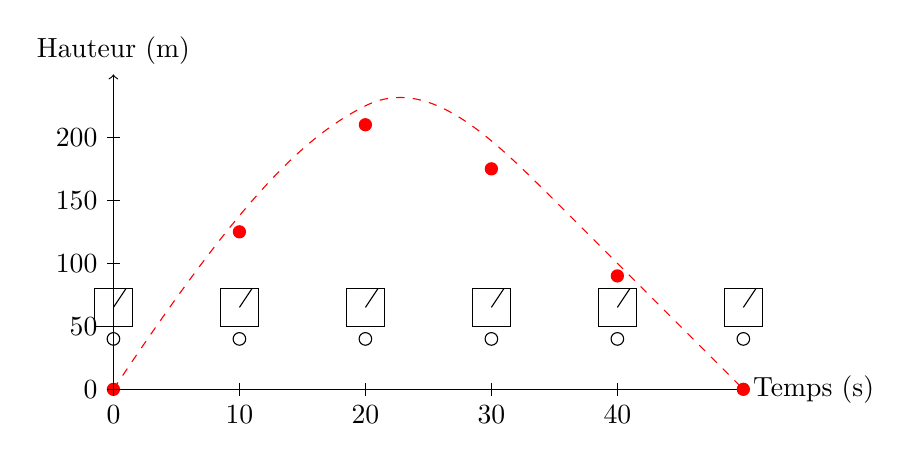
\begin{tikzpicture}[scale=0.8]
  % Axes
  \draw[->] (0,0) -- (10,0) node[right] {Temps (s)};
  \draw[->] (0,0) -- (0,5) node[above] {Hauteur (m)};
  % Courbe en pointillés
  \draw[red, dashed] 
    (0,0) .. controls (2,3) and (3,4) .. (4,4.5)
           .. controls (5,5) and (6,4) .. (7,3)
           .. controls (8,2) and (9,1) .. (10,0);
  % Points d'échantillonnage
  \foreach \x/\y in {0/0,2/2.5,4/4.2,6/3.5,8/1.8,10/0}
    \fill[red] (\x,\y) circle (3pt);
  % Appareils photo
  \foreach \x in {0,2,4,6,8,10} {
    \draw (\x, \y + 0.8) ++(-0.3,0.2) rectangle ++(0.6,0.6);
    \draw (\x, \y + 0.8) ++(0,0.5) -- ++(0.2,0.3);
    \draw (\x, \y + 0.8) circle (0.1);
  }
  % Graduations
  \foreach \x/\label in {0/0,2/10,4/20,6/30,8/40}
    \draw (\x,0.1) -- (\x,-0.1) node[below] {\label};
  \foreach \y/\label in {0/0,1/50,2/100,3/150,4/200}
    \draw (0.1,\y) -- (-0.1,\y) node[left] {\label};
\end{tikzpicture}

\vspace{0.5em}
\textbf{Légende :} L’échantillonnage, c’est comme prendre des \textbf{photos du son} toutes les 10 secondes. On garde un point toutes les 10 s.

\vspace{1em}
\textbf{À colorier :}
\begin{itemize}[leftmargin=*]
  \item Les points ● en \textbf{rouge foncé}.
  \item Les appareils photo
